% 6-8 pages !
% Propose and substantiate managerial, business and organisational solutions to the key problem(s):
% Proposals shall be prospective aiming at providing robust solutions to address the key problem(s).
% Remember to discuss the implementation aspect of your solution(s).
% There must be a coherence between the key problem(s), its causes and the proposed solutions.
% It is crucial to develop various alternative proposals for solutions. Select and motivate which proposals you think would best address the key problem.
% Use models and theories to support your proposals addressing organisational changes, changes of business model etc.
In the following section, the solution propositions that aim to address the previously found issues are explored. In order to have a good overview over which solution resolves which problem, we constructed a matrix which can be found in figure \ref{fig:solution}.

\subsection{Reworking the marketing strategy}

A marketing strategy is a long-term, forward-looking approach with the fundamental goal of achieving a sustainable competitive advantage. By analyzing the Star Model, Business Canvas Model and Porters generic strategies we found some problems which could be improved by changing the current marketing strategy of Howdy, which may lead the customers to on-board HOWDY to a greater extend.

\noindent Analyzing all the information which are given to us, we made some assumptions on which we studied and structured some solutions which are given bellow:

\noindent \textbf{Establish an Effective sales and Marketing team}  $|$ According to the results from the previous sections, it has been identified that the companys current sales team is inefficient and from the company presentation it was revealed that daily tasks intervene with strategy meetings. This may lead to why the company have been losing money over the past years. So HOWDY can establish a strong sales and marketing team by recruiting some efficient personnel who will continuously monitor the sales progress and implement the correct and fruitful marketing strategy for the betterment of the organization. The sales and marketing manager will also manage both the marketing and the sales staff and will perform managerial duties to meet the operational goals of the company.

\noindent \textbf{Put more efforts in advertising HOWDY} $|$ From analyzing previous data we can see that Howdy is advertising their product in a limited way through their partners. Since this has been a detriment to their profit margins and grown their client list at a slow pace, we believe it is better to shift the marketing focus on to other channels.

\begin{enumerate}
    \item Use LinkedIn the right way $|$ As HOWDY is a B2B IT based organization, keeping a connection on LinkedIn will lead them to be connected with other organizations and IT professionals. Howdy can reach a large audience by introducing a strong profile presenting their business through LinkedIn.
    \item Use Email Marketing $|$ Email marketing is still a very effective marketing tactic with a relatively low cost and high ROI. Through Email marketing HOWDY can educate it’s audience about their products and services and invite the audience to attend offline events or webinars.
    \item Telemarketing $|$ Howdy have already adopted telemarketing in their marketing strategy but increasing the focus on this could help as they diverge from relying on partners.
\end{enumerate}

\noindent \textbf{Introduce free Workshops and Webinars} $|$ People love new learning experiences so it could be a good idea for HOWDY to introduce some workshops or webinars related to it’s products or services. Many business organizations may get attracted to on-boarding HOWDY through this channel.

\noindent \textbf{Customer Surveys} $|$ In order to get an insight into the reasons why Howdys marketing strategy is failing they can implement quick customer surveys. Then they can utilize an analytical tool to determine the aspects of their strategy that are not working and show which marketing channels are bringing in the bulk of traffic and which are not. They may also implement surveys to see how customers are finding their business. Once they have this information, they can use it to their advantage

\subsection{Organisational restructuring}
In order for Howdy to divert from their current path and grow their business a change in the organizational structure could be beneficial.

\noindent As mentioned in the previous section the marketing and sales of the company could improve by expanding the sales team so it will not be discussed here.

\noindent Howdy also has the problem of the development being interrupted by day-to-day tasks like maintenance. As the development is of significant importance it would benefit Howdy to address this problem.\\
\noindent One way of doing this is by expanding the maintenance team until the workload does not surpass the resources of the team.\\
\noindent If expanding the team is not viable then another option could be to assign someone working with development to the maintenance team. This will slow the development but the continuous operation of the company is more important and the rest of the developers will also be able to fully focus on their assigned tasks. As the maintenance workload might change every day the people who previously worked with development would still be able to support the developers when the workload is small.

\noindent Even though the cost of Howdys´ product is not identified as a problem in the retrospective analysis it could still increase resources for solutions to the problems presented in this document or for other activities. One of the significant costs for Howdy is the external psychologists they hire as part of their service. It is not known what the workload for this task is but hiring their own psychologists could reduce costs as an internal psychologist costs less than 50\% of what an external one does according to the CEO of Howdy\cite{q&a}.

%%
%% Reworking the pricing system
%%   -- Jesper --
%%
\subsection{Revamping the pricing system}
The perfect pricing system shares information to the customer to help them decide which product to chose. A pricing table must share the right amount of information without sharing too much as this often will result in chaotic pricing tables. Our proposed pricing table solution for Howdy can be seen on figure [\ref{pricingtable}] below.

\begin{figure}[H]
\centering
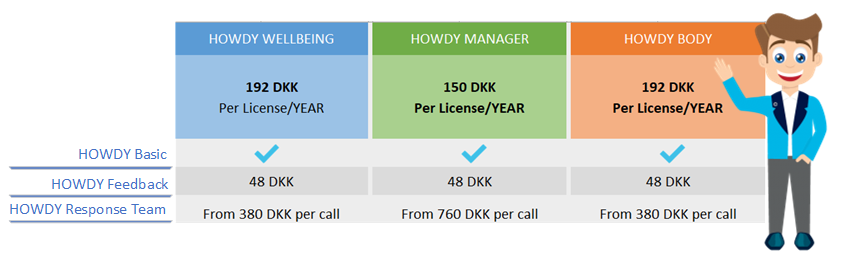
\includegraphics[scale=0.72]{figures/pricing_Howdy.png}
\caption{Howdys´ new pricing table}
\label{pricingtable}
\end{figure}

\noindent In the old pricing table Howdy also had important information hidden as small text in lesser visual areas, an example would be in the top left corner where it says per license \cite[p.30]{oneofthepresentations}. Furthermore Howdy also chose to put the cost per call in small text under the module names making it hard for customers to initially see the actual price. 

\noindent The new pricing table is way less chaotic and some of the reason for this is that we included Howdy Basic, which is the mandatory it-system, in all the packages as Howdy cannot be used without. The inclusion of Howdy Basic in reflected in the price and visually shown with a Howdy blue colored check mark. The necessary information and cost estimate is now more clear for the customer and will be less intimidating.


\noindent Howdy currently has discount for mass purchases as can be seen when buying points for calls. At the moment our proposed pricing table solution states a price for Howdy Response Team but it might as well display the point cost as the current price is calculated based on the large point package. By keeping points instead of static numbers for the cost of Response Team calls, Howdy will still be able to offer discount on mass purchases. Furthermore Howdy should also consider offering discounts for mass purchases of their licenses, making it more attractive for larger companies to include all their employees when on-boarding a Howdy product. 

\subsection{Solution matrix}

In order to asses the usefulness of each of our proposed solutions, we have created a solution matrix, attached in figure \ref{fig:solution}. Our proposed solution are mostly aimed at solving the inefficient marketing strategy, as this will be the fastest way of putting Howdy back on track in regards to earning a profit.

\begin{figure}[H]
\centering
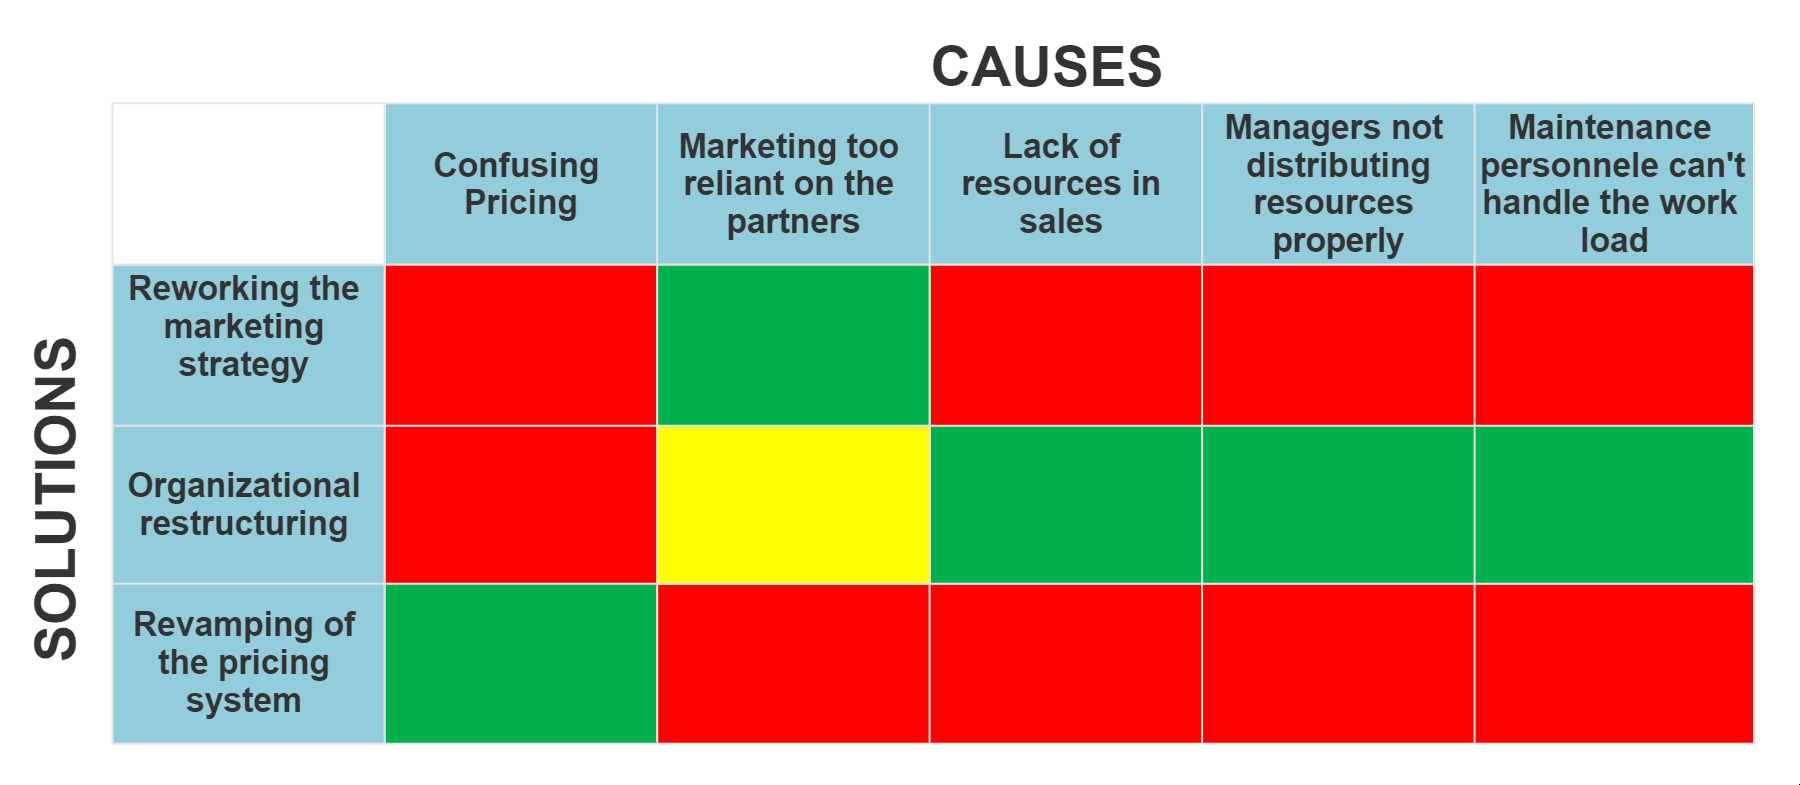
\includegraphics[width=0.95\textwidth]{figures/solutionmatrix .png}
\caption{Solution matrix. Where green means that the solution addresses the cause, yellow means that it helps and red means that it does not solve the cause}
\label{fig:solution}
\end{figure}
